% ===========================
%       Chapter 1A.2
%      Carbohydrates:
%   Mono- and Disaccharides
%   Created by Michael Tang
%        2024.12.30
% ===========================

\subsubsection{1A.2 Carbohydrates: Monosaccharides and Disaccharides}
\paragraph{What are Organic Compounds?}
\begin{itemize}
    \item \textbf{Definition:} Organic compounds are molecules containing carbon atoms bonded to hydrogen and other elements, such
    as oxygen, nitrogen, and phosphorus. In some carbon compounds small molecules (\underline{monomers} 单体) bond with many
    other similar units to make a very large molecule called a \underline{polymer} (聚合物). The ability of carbon to combine and
    make \underline{macromolecules} (大分子) is the basis of all biological molecules and provides the great variety and
    complexity found in living things.
    \begin{figure}[H]
        \centering
        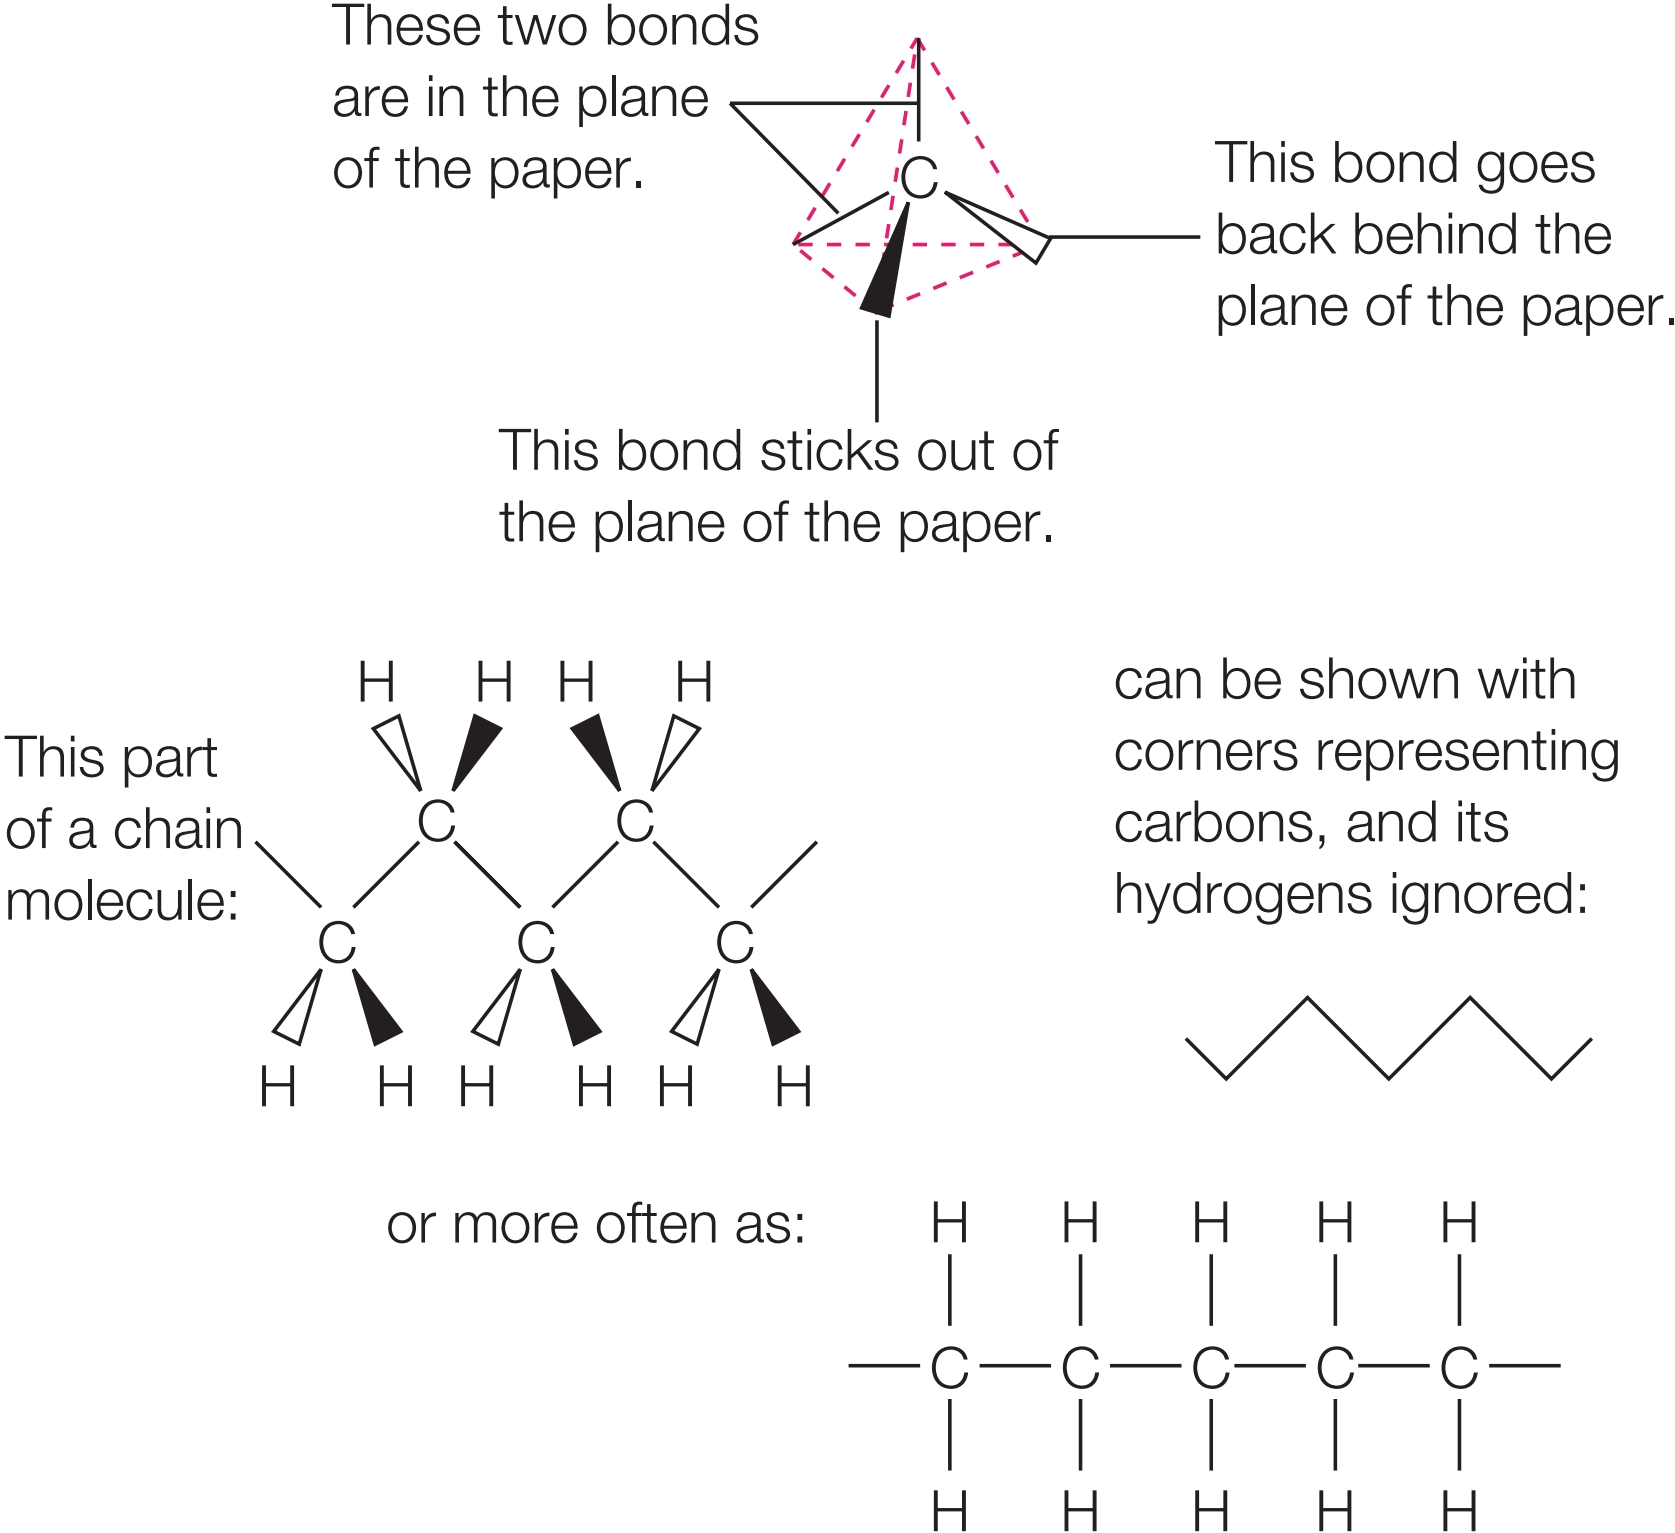
\includegraphics[scale=0.18]{Biology/1A/Images/1A-2-1.png}
        \caption{The bonds in a carbon atom have a complicated 3D shape. This is difficult to represent, so in most molecular
        diagrams we use one of several different ways to draw them.}
    \end{figure}
    \item \textbf{Key Features:}
    \begin{itemize}
        \item Carbon atoms form stable covalent bonds, allowing complex structures.
        \item Organic compounds include \underline{carbohydrates} (碳水化合物), \underline{lipids} (脂质), \underline{proteins}
        (蛋白质), and \underline{nucleic acids} (核酸).
    \end{itemize}
\end{itemize}

\paragraph{Carbohydrates}
Carbohydrates are essential organic molecules, primarily serving as energy sources and structural components. They are composed
of carbon (\ce{C} 碳), hydrogen (\ce{H} 氢), and oxygen (\ce{O} 氧), typically in a 1:2:1 ratio - \ce{(CH2O)_n}.

\paragraph{\underline{Monosaccharides} (单糖): The Simplest Sugars}
\begin{itemize}
    \item \textbf{Key Characteristics:}
    \begin{itemize}
        \item Simplest form of carbohydrates.
        \item General formula: \ce{(CH2O)_n}, where $n$ is the number of carbon. Although $n$ can be any number, but it
        is usually low (3-7).
        \item Examples:
        \begin{itemize}
            \item \textbf{Triose (3-Carbon 三糖, $n=3$):} \ce{C3H6O3}. E.g., \underline{glyceraldehyde} (甘油醛), involved in
            \underline{glycolysis} (糖酵解).
            \item \textbf{Pentose (5-Carbon 五糖, $n=5$):} \ce{C5H10O5}. E.g., \underline{ribose} (核糖) and
            \underline{deoxyribose} (脱氧核糖).
            \begin{figure}[H]
                \centering
                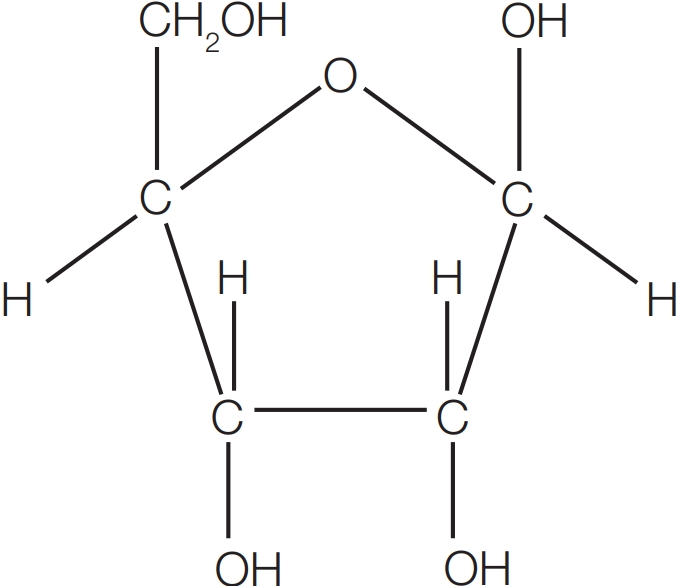
\includegraphics[scale=0.25]{Biology/1A/Images/1A-2-2.png}
                \caption{Pentose sugars such as ribose have 5 carbon atoms.}
            \end{figure}
            \item \textbf{Hexose (6-Carbon 六糖 , $n=6$):} \ce{C6H12O6}. E.g., glucose (energy source 葡萄糖), fructose (fruit
            sugar 果糖), galactose (milk sugar 半乳糖).
        \end{itemize}
        \item Structure of Glucose
        \begin{itemize}
            \item Gulcose has two \underline{isomers} (different forms 同分异构体): $\alpha$-glucose and $\beta$-glucose. The two
            isomers have different arrangements of the atoms on the side chains of the molecule.
            \item \textbf{Alpha($\alpha$) glucose:} \underline{Hydroxyl} (\ce{-OH} 羟基) group on carbon 1 is below the plane.
            \item \textbf{Beta($\beta$) glucose:} Hydroxyl group on carbon 1 is above the plane.
        \end{itemize}
        \begin{figure}[H]
            \centering
            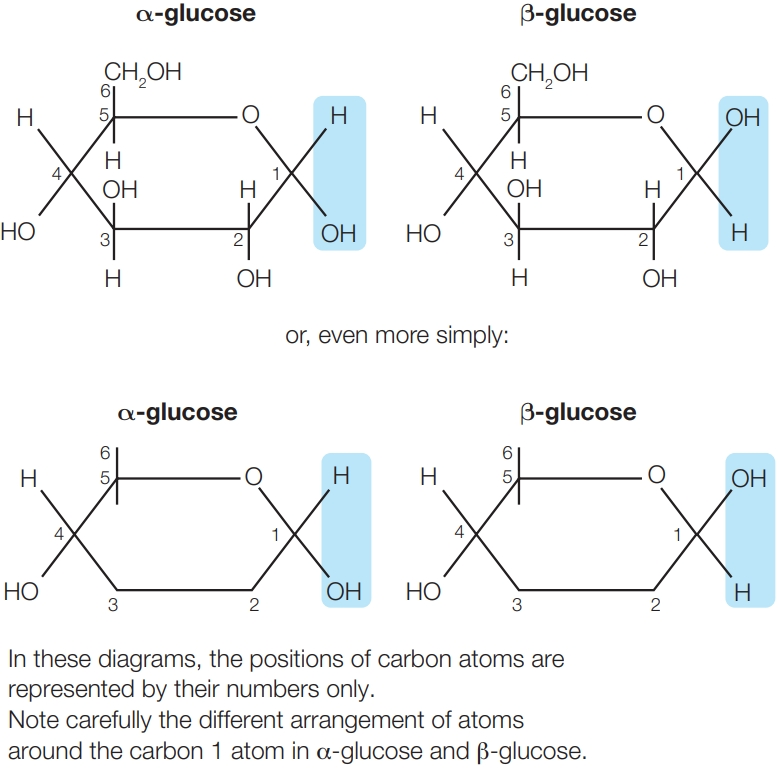
\includegraphics[scale=0.155]{Biology/1A/Images/1A-2-3.png}
            \caption{Hexose sugars have a ring structure. The arrangement of the atoms on the side chains can make a significant
            difference to the way in which the molecule can be used by the body. The carbon atoms are numbered in order to
            identify the different arrangements.}
        \end{figure}
    \end{itemize}
\end{itemize}

\paragraph{\underline{Disaccharides} (二糖): The Double Sugars}
\begin{itemize}
    \item \textbf{Formation:}
    \begin{itemize}
        \item \textbf{\underline{Condensation Reaction} (缩合反应):} Two monosaccharides join, forming a \underline{glycosidic
        bond} (糖苷键) and releasing a water molecule (\ce{H2O}).
        \begin{figure}[H]
            \centering
            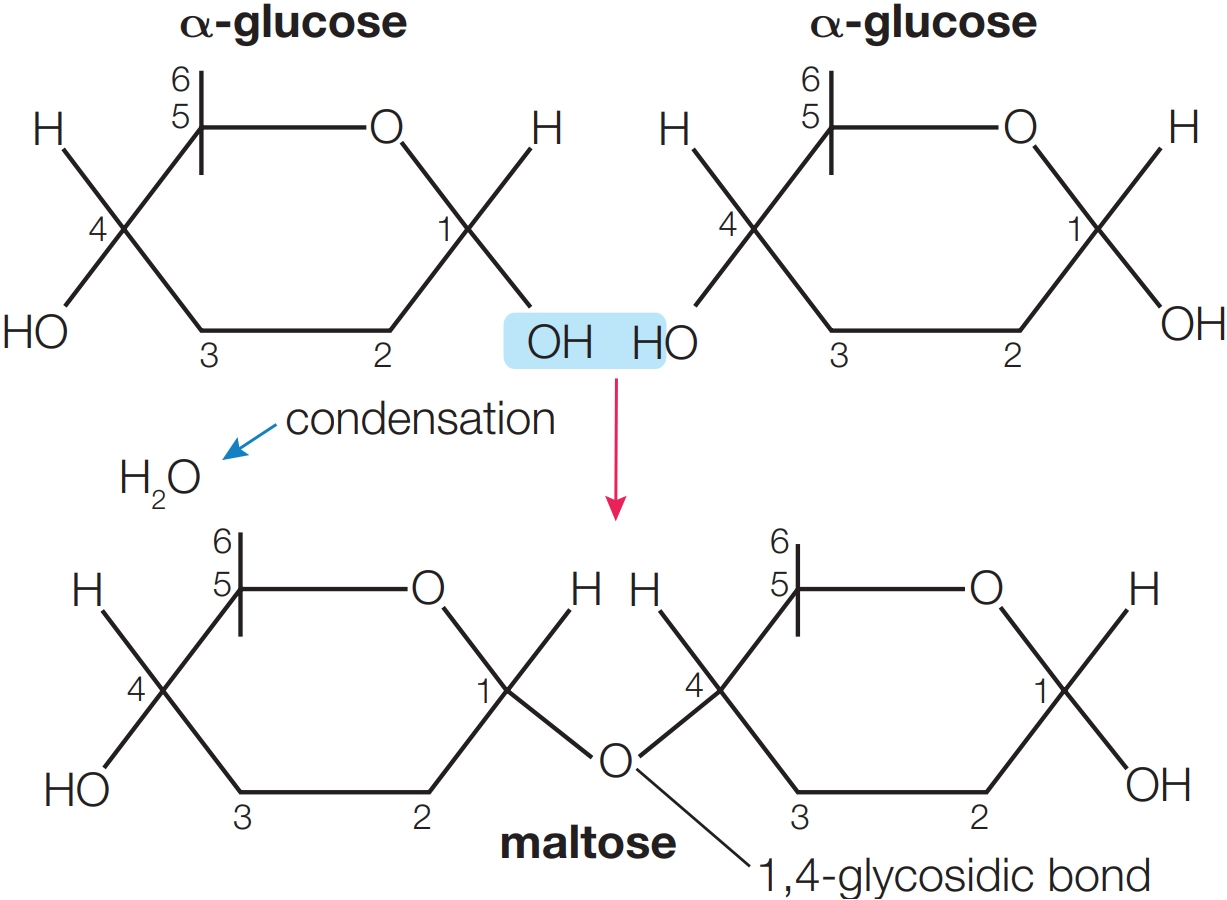
\includegraphics[scale=0.18]{Biology/1A/Images/1A-2-4.png}
            \caption{The formation of a glycosidic bond. The condensation reaction between two monosaccharides results in a
            disaccharide and a molecule of water.}
        \end{figure}
        \item \textbf{Examples:}
        \begin{itemize}
            \item \textbf{\underline{Sucrose} (蔗糖):} Glucose + Fructose. Stored in plants such as \underline{sugar cane} (甘蔗).
            \item \textbf{\underline{Lactose} (乳糖):} Glucose + Galactose. Milk sugar - this is the main carbohydrate found in
            milk.
            \item \textbf{\underline{Maltose} (麦芽糖):} Glucose + Glucose. \underline{Malt} (麦芽) sugar - found in
            \underline{germinating} (发芽) seed such as \underline{barley} (大麦).
        \end{itemize}
    \end{itemize}
    \item \textbf{Breakdown - \underline{Hydrolysis Reaction} (水解反应):} Glycosidic bonds are broken with the
    \underline{addition} (添加) of water, \underline{yielding} (产生) two monosaccharides.
\end{itemize}

\paragraph{Testing for Sugars - \underline{Benedict's Test} (本尼迪克特试验)}
\begin{itemize}
    \item \textbf{Principle:} Benedict's test is a \underline{qualitative test} \footnote{\textbf{Qualitative Test:} A qualitative
    test determines the \underline{presence} (存在) or \underline{absence} (不存在) of a specific substance in a sample, without
    providing \underline{precise} (精确的) numerical data about its \underline{concentration} (浓度) or \underline{quantity} (数量)
    \begin{itemize}
        \item \textbf{Key Features:}
        \begin{itemize}
            \item \textbf{Purpose:} Identify whether a substance is present.
            \item \textbf{Outcome:} Results are typically \underline{descriptive} (描述性的 - e.g., color change, precipitation
            沉淀, or effervescence 泡沫) rather than \underline{quantitative} (定量性的).
            \item \textbf{Examples in Biology and Chemistry:} Benedict's test for reducing sugars (color change from blue to
            brick-red), iodine test for starch (color change from yellow-brown to blue-black), and \underline{biuret test}
            (缩二脲试验) for proteins (color change from blue to purple).
        \end{itemize}
        \item \textbf{Limitations:}
        \begin{itemize}
            \item Does not measure the exact amount of a substance.
            \item \underline{Subjective interpretation} (主观解释)  of results (e.g., intensity of color change 颜色变化的程度).
        \end{itemize}
    \end{itemize}} (定性实验) used to detect the presence of \underline{reducing sugars} (还原糖). These sugars can reduce copper
    (II) ions (\ce{Cu^2+}) to copper (I) ions (\ce{Cu^+}) due to the presence of a free \underline{aldehyde} (\ce{R-CHO} \footnote{In
    organic chemistrym \ce{R} is a \underline{shorthand symbol} (缩写符号) used to represent a generic \underline{alkyl group} (烷基)
    or \underline{side chain} (侧链) attached to a \underline{functional group} \footnotemark[9] (官能团). It is a
    \underline{placeholder} (占位符) for any group of carbon and hydrogen atoms (and sometimes other atoms) in a molecule.
    \begin{itemize}
        \item \textbf{Explanation of \ce{R} in \ce{R-CHO}:}
        \begin{itemize}
            \item \ce{R}: Represents a \underline{hydrocarbon} (烃/碳氢化合物) chain or group, such as:
            \begin{itemize}
                \item \underline{Methyl group} (甲基): \ce{CH3-}
                \item \underline{Ethyl group} (乙基): \ce{CH3CH2-}
                \item \underline{Cycloalkyl group} (环烷基): \ce{C6H11}
                \item Longer or branched alkyl chains: \ce{C_nH_{2n+1}}
            \end{itemize}
            \item \ce{CHO}: Represents the \underline{aldehyde functional group} (醛官能团), where a carbon atom is
            \underline{double-bonded} (双键) to an oxygen atom (\ce{C=O}) and \underline{single-bonded} (单键) to a hydrogen atom
            (\ce{H}).
        \end{itemize}
        \item \textbf{Purpose of \ce{R}:}
        \begin{itemize}
            \item[1.] \textbf{Generic Representation:} It simplifies chemical structures when the specific nature of the alkyl
            group is not important for the discussion.
            \item[2.] \textbf{Flexibility:} Allows focus on the functional group (\ce{CHO}) rather than the details of the alkyl
            chain.
        \end{itemize}
        \item \textbf{Examples:} Methanal (Formaldehyde 甲醛): \ce{H-CHO}, where \ce{R=H}.
    \end{itemize}} 醛) or
    \underline{ketone} (\ce{R-CO-R}$'$ \footnote{\ce{R-CO-R}$'$ can also write as $>$\ce{C=O}. In organic chemistry, the symbol $>$\ce{C=O} is used
    to describe the structure of a \underline{carbonyl group} (羰基), emphasizing that the carbon atom in the carbonyl group is
    bonded not only to an oxygen atom but also to two other \underline{groups} (基团). The $>$ symbol indicates that the carbonyl
    carbon is an \underline{internal carbon} (内部碳), connected to two other groups or chains (rather than being a terminal
    carbon).} 酮) group.
    \footnotetext[9]{\textbf{Functional group:} A functional group is a specific group of atoms within a molecule that
    determines the chemical properties and reactions of that molecule. It is the reactive part of the molecule, often defining
    its behavior in biological or chemical processes. Functional groups are crucial in organic chemistry because they dictate how
    molecules interact and bond with others.}
    \item \textbf{Reducing sugars:} Reducing sugars include monosaccharides like glucose, furctose, and galactose, and
    disaccharides except sucrose. They have the ability to donate electrons to other molecules due to their reactive carbonyl
    group.
    \item \textbf{Reagents in Benedict's Test:} Benedict's Solution contains:
    \begin{itemize}
        \item \textbf{Copper (II) Sulfate (\ce{CuSO4}):} Source of (\ce{Cu^2+}) ions.
        \item \textbf{Sodium Citrate (\ce{C6H5Na3O7}):} Stablizes the copper (II) ions in the solution.
        \item \textbf{Sodium Carbonate (\ce{Na2CO3}):} Provides an alkaline environment.
    \end{itemize}
    \item \textbf{Chemical Reaction:}
    \begin{itemize}
        \item[1.] In an alkaline medium, the carbonyl group of the reducing sugar reacts with the copper (II) ions.
        \item[2.] Reduction Process:
        \begin{itemize}
            \item \ce{Cu^2+} (blue) is reduced to \ce{Cu^+} (red/orange precipitate of copper (I) oxide, \ce{Cu2O}).
            \item Reaction:
            \begin{equation}
                \ce{R-CHO + 2Cu^2+ + 5OH^- -> R-COOH + Cu2O + 2H2O}
            \end{equation}
            Where \ce{R-CHO} represents the reducing sugar.
        \end{itemize} 
    \end{itemize}
    \item \textbf{Procedure:}
    \begin{itemize}
        \item[1.] Mix the sample with Benedict's solution.
        \item[2.] Heat the mixture in a boiling water bath for about 2-5 minutes.
        \item[3.] Observe the color change and precipitate formation.
    \end{itemize}
    \item \textbf{Observation and Results:}
    \begin{table}[h!]
        \centering
        \begin{tabular}{|l|l|}
        \hline
        \textbf{Color Change}          & \textbf{Reducing Sugar Concentration} \\ \hline
        Blue (no change)               & No reducing sugar present             \\ \hline
        Green                          & Low concentration                     \\ \hline
        Yellow                         & Moderate concentration                \\ \hline
        Brick-red precipitate          & High concentration                    \\ \hline
        \end{tabular}
        \caption{Color changes observed in Benedict's test for reducing sugars.}
        \label{tab:reducing_sugars}
    \end{table}
    \begin{figure}[H]
        \centering
        \includegraphics[scale=1]{Biology/1A/Images/1A-2-5.bmp}
        \caption{Benedict's test for reducing sugars.}
    \end{figure}
    \item \textbf{Limitations:} Non-reducing sugars like sucrose do not react directly unless hydrolyzed.
\end{itemize}